\begin{figure}[H]
	\centering
	\begin{subfigure}{.6\linewidth}
		\centering
		\tikzset{rod/.style={cylinder, draw, shape aspect=.5,
					cylinder uses custom fill, cylinder end fill=black!50,
					minimum height=60,
					cylinder body fill=black!20,
					scale=2, rotate=200,anchor=east}
		}
		\begin{tikzpicture}
			% Rod bottom + left
			\node[rod] (rb) at (0,-0.5,0) {}; % bottom
			\node[rod] (rl) at (-0.5,0,-0.5) {}; % left
			% Beam
			\draw[red,arrows = {-Stealth},rotate=20] (-1,0) node[black,anchor=north,rotate=20] {Ionkilde} -- (0,0) sin +(.2,.2) cos +(.2,-.2) sin +(.2,-.2) cos +(.2,.2) sin +(.2,.2) cos +(.2,-.2) sin +(.2,-.2) cos +(.2,.2) sin +(.2,.2) cos +(.2,-.2) sin +(.2,-.2) cos +(.2,.2) sin +(.2,.2) cos +(.2,-.2) sin +(.2,-.2) cos +(.2,.2) sin +(.2,.2) cos +(.2,-.2) sin +(.2,-.2) cos +(.2,.2) sin +(.2,.2) cos +(.2,-.2) -- +(1,0) node[black,anchor=south,rotate=20] {Detektor};
			% Rod top
			\node[rod] (rt) at (0,0.5,0) {}; % top
			% Rod see through
			\node[rod,minimum height=6] (rr1) at (0.5,0,0.5) {}; % right 1
			\node[rod,minimum height=6,xshift=-50,cylinder end fill=black!20] (rr2) at (0.5,0,0.5) {}; % right 2
			\draw[dashed] (rr1.after bottom) -- (rr2.before top);
			\draw[dashed] (rr1.before bottom) -- (rr2.after top);
			% Firpol text
			\node[anchor=south,yshift=15,rotate=20] at (rt.north east) {Firpol};
		\end{tikzpicture}
		\caption{Diagram over firpol. Den røde bane viser banen af et stabilt molekyle, som altså har den rette $m/z$.}
		\label{fig:quadpolebig}
	\end{subfigure}\hspace{.05\linewidth}%
	\begin{subfigure}{.3\linewidth}
		\centering
		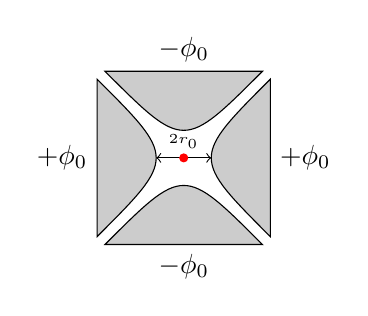
\begin{tikzpicture}
			\draw[fill=black!20] (-1,1.1) .. controls (0,.1) .. (1,1.1) -- cycle;
			\draw[fill=black!20] (-1,-1.1) .. controls (0,-.1) .. (,-1.1) -- cycle;
			\begin{scope}[rotate=90]
				\draw[fill=black!20] (-1,1.1) .. controls (0,.1) .. (1,1.1) -- cycle;
				\draw[fill=black!20] (-1,-1.1) .. controls (0,-.1) .. (1,-1.1) -- cycle;
			\end{scope}

			\node[anchor=south] at (0,1.1) {$-\phi_0$};
			\node[anchor=north] at (0,-1.1) {$-\phi_0$};
			\node[anchor=east] at (-1.1,0) {$+\phi_0$};
			\node[anchor=west] at (1.1,0) {$+\phi_0$};

			\draw[<->] (-.35,0) -- (0,0) node[anchor=south] {\tiny$2r_0$} -- (.35,0) ;

			\filldraw[red] (0,0) circle (0.05);
		\end{tikzpicture}
		\caption{Snit af firpol, med potentialerne $\phi_0 = U - V \cos{\omega t}$.}
		\label{fig:quadpolecharge}
	\end{subfigure}
	\caption{Diagram over firpolet MS, med snit som viser potentialerne i stængerne. \parencite{massspec}}
	\label{fig:quadpole}
\end{figure}
